\documentclass[a4paper]{article}
\usepackage{color}              %Farben, f.r \definecolor{}
\usepackage{amssymb}            %Mathematische Symbole
\usepackage{amsthm}             %Besseres \newtheorem
\usepackage{amsmath}           %Mathematische Umgebungen
\usepackage{mathtools}          %\xRightarrow, etc
\usepackage{mathrsfs}           %enthaelt \mathscr
\usepackage{graphicx}
\usepackage{enumerate}          % in-place numerations def.
\usepackage{fullpage}

\usepackage{array}
%\usepackage{multicol}
%\usepackage[notref,notcite]{showkeys}
%\usepackage{algorithm,algorithmic}
\usepackage{color}

\usepackage{graphicx}
\usepackage{xypic}
\entrymodifiers={+!!<0pt,\fontdimen22\textfont2>}
\usepackage[all]{xy}

\usepackage{float}
\usepackage{tikz}
\usepackage{tikz-cd}
\usepackage{tikz,fullpage}
\usetikzlibrary{arrows,%
                petri,%
                topaths}%
\usepackage{tkz-berge}
\usepackage[position=top]{subfig}
\usetikzlibrary{shapes.geometric}
\usetikzlibrary{decorations.markings}
\usetikzlibrary{graphs}

\newtheoremstyle{myremark} % name
    {7pt}                    % Space above
    {7pt}                    % Space below
    {}  	                 % Body font
    {}                           % Indent amount
    {\bf}       	         % Theorem head font
    {.}                          % Punctuation after theorem head
    {.5em}                       % Space after theorem head
    {}  % Theorem head spec (can be left empty, meaning ‘normal’)

\theoremstyle{plain}
\newtheorem{lemma}{Lemma}
\newtheorem{theorem}[lemma]{Theorem}
\newtheorem{fact}[lemma]{Fact}
\newtheorem{definition}[lemma]{Definition}
\newtheorem{corollary}[lemma]{Corollary}
\newtheorem{proposition}[lemma]{Proposition}
\newtheorem{conjecture}[lemma]{Conjecture}
\newtheorem{observation}[lemma]{Observation}
\newtheorem{problem}[lemma]{Problem}
\newtheorem{notation}[lemma]{Notation}
\newtheorem*{claim}{Claim}

\theoremstyle{myremark}
\newtheorem{remark}[lemma]{Remark}
\newtheorem{example}[lemma]{Example}
\newtheorem{exercise}[lemma]{Exercise}
\newtheorem{algorithm}[lemma]{Algorithm}
\newtheorem{application}[lemma]{Application}
\newtheorem*{goal}{Goal}

%%%%%% EDIT HERE: %%%%%%%%%%%
\newcommand{\LECTURENUMBER}{0}
\newcommand{\LECTURETITLE}{Short title}
\newcommand{\LECTURESCRIBE}{Your name}

%% Dokument Beginn %%%%%%%%%%%%%%%%%%%%%%%%%%%%%%%%%%%%%%%%%%%%%%%%%%%%%%%%
\begin{document}
\thispagestyle{empty}

\begin{center}
	{\Large\bf Graph coloring}\\
	{\bf Lecture notes, vol. 5 \\ Planar Graphs}\\
\end{center}
Lecturer: Michal Adamaszek \hfill Scribe: Sokratis Theodoridis
\begin{center}
\line(1,0){450}
\end{center}

%%%%%%% EDIT ALSO BELOW: %%%%%%%%%%%%%%%%
 
\begin{definition}
$G$ is \emph{planar} if it can be drawn on ${\rm I\!R^2}$(the plane) so that edges intersect only at their common endpoints.
We call such a drawing an \emph{"embedding"}(some authors say \emph{"drawing"}).
\end{definition}

\begin{example}

\begin {tikzpicture}

\draw   
           node[fill,circle,inner sep=0pt,minimum size=3pt] (n1) at (0,0) {}
	node[fill,circle,inner sep=0pt,minimum size=3pt] (n2) at (1,0) {} 
	node[fill,circle,inner sep=0pt,minimum size=3pt] (n3) at (0,1) {} 
	node[fill,circle,inner sep=0pt,minimum size=3pt] (n4) at (1,1) {}
[line width = 1 pt, black, -] (n1) edge (n4)
[line width = 1 pt, black, -] (n2) edge (n3)
[line width = 1 pt, black, -] (n1) edge (n2)
[line width = 1 pt, black, -] (n2) edge (n4)
[line width = 1 pt, black, -] (n4) edge (n3)
[line width = 1 pt, black, -] (n3) edge (n1)
;
\end{tikzpicture}
       $K_4$ not an embedding
\begin {tikzpicture}
\newcommand*{\OutAngle}{60}
 \newcommand*{\ArcMax}{1.2}
\draw
	node[fill,circle,inner sep=0pt,minimum size=3pt] (n1) at (0,0) {}
	node[fill,circle,inner sep=0pt,minimum size=3pt] (n2) at (1,0) {} 
	node[fill,circle,inner sep=0pt,minimum size=3pt] (n3) at (0,1) {} 
	node[fill,circle,inner sep=0pt,minimum size=3pt] (n4) at (1,1) {}
[line width = 1 pt, black, -] (n1) edge (n2)
[line width = 1 pt, black, -] (n1) edge (n2)
[line width = 1 pt, black, -] (n2) edge (n4)
[line width = 1 pt, black, -] (n4) edge (n3)
[line width = 1 pt, black, -] (n3) edge (n1)
(0, 1) to[out=\OutAngle, in=135]
    (\ArcMax, \ArcMax) to[out=-45, in=90-\OutAngle]
    (1, 0) -- cycle
;
\end{tikzpicture}
embedding ($K_4$ is planar)
\newline
\newline
\begin {tikzpicture}
\draw 
%node[fill,circle,inner sep=0pt,minimum size=3pt] (n1) at (0,0) {}
node[fill,circle,inner sep=0pt,minimum size=3pt] (n2) at (-0.5,0) {}
node[fill,circle,inner sep=0pt,minimum size=3pt] (n3) at (0,0.5) {}
node[fill,circle,inner sep=0pt,minimum size=3pt] (n4) at (0.5,0) {}
node[fill,circle,inner sep=0pt,minimum size=3pt] (n5) at (0,1) {}
[line width = 1 pt, black, -] (n2) edge (n4)
%[line width = 1 pt, black, -] (n1) edge (n4)
[line width = 1 pt, black, -] (n3) edge (n5)
[line width = 1 pt, black, -] (n2) edge (n5)
[line width = 1 pt, black, -] (n4) edge (n5)
[line width = 1 pt, black, -] (n3) edge (n4)
[line width = 1 pt, black, -] (n2) edge (n3)
;
\end{tikzpicture}
straight line-embedding
\end{example}

\begin{theorem}(F{\'a}ry,\emph{1948}) If $G$ has an embedding, then it also has one where every edge is a straight line segment.
\end{theorem}
\begin{remark} $G$ can be treated as a topological space [($CW-$,$\Delta-$,simplicial-) complex]. Then $G$ is planar if (as a topological space) it embeds into ${\rm I\!R^2}$ ($embedding \equiv continuous, injective\ map$)
\end{remark}

\begin{example}
\begin {tikzpicture}
\draw  
	node[fill,circle,inner sep=0pt,minimum size=3pt] (n1) at (0,0) {}
	node[fill,circle,inner sep=0pt,minimum size=3pt] (n2) at (-1,0) {}
	node[fill,circle,inner sep=0pt,minimum size=3pt] (n3) at (1,0) {}
	node[fill,circle,inner sep=0pt,minimum size=3pt] (n4) at (0,-1) {}
	node[fill,circle,inner sep=0pt,minimum size=3pt] (n5) at (-1,-1) {}
	node[fill,circle,inner sep=0pt,minimum size=3pt] (n6) at (1,-1) {}
[line width = 1 pt, black, -] (n2) edge (n5)
[line width = 1 pt, black, -] (n2) edge (n4)
[line width = 1 pt, black, -] (n2) edge (n6)
[line width = 1 pt, black, -] (n1) edge (n5)
[line width = 1 pt, black, -] (n1) edge (n6)
[line width = 1 pt, black, -] (n1) edge (n4)
[line width = 1 pt, black, -] (n3) edge (n4)
[line width = 1 pt, black, -] (n3) edge (n5)
[line width = 1 pt, black, -] (n3) edge (n6);
\end {tikzpicture}
{$K_{3,3}$}
\begin {tikzpicture}
\draw
node[fill,circle,inner sep=0pt,minimum size=3pt] (n1) at (0,0) {}
(0,0) node [text=black,above] {$2$}
node[fill,circle,inner sep=0pt,minimum size=3pt] (n2) at (-1,0) {}
(-1,0) node [text=black,above] {$1$}
node[fill,circle,inner sep=0pt,minimum size=3pt] (n3) at (-1.5,-1) {}
(-1.5,-1) node [text=black,below] {$5$}
node[fill,circle,inner sep=0pt,minimum size=3pt] (n4) at (0.5,-1) {}
(0.5,-1) node [text=black,below] {$3$}
node[fill,circle,inner sep=0pt,minimum size=3pt] (n5) at (-0.5,-1.5) {}
(-0.5,-1.5) node [text=black,below] {$4$}
[line width = 1 pt, black, -] (n2) edge (n5)
[line width = 1 pt, black, -] (n2) edge (n4)
[line width = 1 pt, black, -] (n1) edge (n5)
[line width = 1 pt, black, -] (n3) edge (n5)
[line width = 1 pt, black, -] (n4) edge (n5)
[line width = 1 pt, black, -] (n4) edge (n1)
[line width = 1 pt, black, -] (n1) edge (n2)
[line width = 1 pt, black, -] (n3) edge (n2)
[line width = 1 pt, black, -] (n3) edge (n1)
[line width = 1 pt, black, -] (n3) edge (n4)
[line width = 1 pt, black, -] (n2) edge (n5)
; 
\end {tikzpicture}
{$K_5$}

\end{example}
\bigskip
\bigskip
\begin{observation}\textbf {\textit{"{$K_5$} is not planar"}}
\end {observation}
\begin{proof}
In any planar embedding the cycle 1-2-3-4-5-1 has to be drawn as a polygon: \newline
We can draw at most 2 non intersecting diagonals inside this polygon. \newline
We can draw at most 2 non intersecting diagonals outside this polygon. \newline
\underline {But} we have to draw 5 diagonals, so that is impossible.
\end{proof}

\begin{observation}\textbf {\textit{"{$K_{3,3}$} is not planar"}}
\end{observation}
\begin {proof}
The 6-cycle has to be drawn as a polygon.\newline
We need edges: 15,26,34\newline
At most 1 can appear inside\newline
At most 1 can appear outside
\end {proof}
\begin {tikzpicture}
\draw
node[fill,circle,inner sep=0pt,minimum size=3pt] (n1) at (0,0) {}
	node[fill,circle,inner sep=0pt,minimum size=3pt] (n2) at (-1,0) {}
	node[fill,circle,inner sep=0pt,minimum size=3pt] (n3) at (1,0) {}
	node[fill,circle,inner sep=0pt,minimum size=3pt] (n4) at (0,-1) {}
	node[fill,circle,inner sep=0pt,minimum size=3pt] (n5) at (-1,-1) {}
	node[fill,circle,inner sep=0pt,minimum size=3pt] (n6) at (1,-1) {}
[line width = 1 pt, black, -] (n2) edge (n6)
[line width = 1 pt, black, -] (n1) edge (n5)
[line width = 1 pt, black, -] (n1) edge (n4)
[line width = 1 pt, black, -] (n3) edge (n4)
[line width = 1 pt, black, -] (n3) edge (n6)
[line width = 1 pt, black, -] (n2) edge (n5);
\end {tikzpicture}
{$C_6$}\begin {tikzpicture}
\draw
node[fill,circle,inner sep=0pt,minimum size=3pt] (n1) at (0,0) {}
(0,0) node [text=black,above] {$4$}
node[fill,circle,inner sep=0pt,minimum size=3pt] (n2) at (-1,0) {}
(-1,0) node [text=black,above] {$1$}
node[fill,circle,inner sep=0pt,minimum size=3pt] (n3) at (-1.5,-0.7) {}
(-1.5,-0.7) node [text=black,below] {$6$}
node[fill,circle,inner sep=0pt,minimum size=3pt] (n4) at (0.6,-0.7) {}
(0.6,-0.7) node [text=black,below] {$2$}
node[fill,circle,inner sep=0pt,minimum size=3pt] (n5) at (0,-1.5) {}
(0,-1.5) node [text=black,below] {$5$}
node[fill,circle,inner sep=0pt,minimum size=3pt] (n6) at (-1,-1.5) {}
(-1,-1.5) node [text=black,below] {$3$}
[line width = 1 pt, black, -] (n1) edge node {} (n2)
[line width = 1 pt, black, -] (n1) edge node {} (n4)
[line width = 1 pt, black, -] (n4) edge node {} (n5)
[line width = 1 pt, black, -] (n5) edge node {} (n6)
[line width = 1 pt, black, -] (n6) edge node {} (n3)
[line width = 1 pt, black, -] (n3) edge node {} (n2)
;
\end {tikzpicture}

\begin {definition}\begin{minipage}[t]{\linewidth}
\begin {itemize}
\item An edge subdivision is the replacement 
\begin {tikzpicture}
\draw 
node[fill,circle,inner sep=0pt,minimum size=3pt] (n1) at (0,0) {}
(0,0) node [text=black,above] {$v$}
node[fill,circle,inner sep=0pt,minimum size=3pt] (n2) at (2,0) {}
(2,0) node [text=black,above] {$w$}
[line width = 1 pt, black, -] (n1) edge node {} (n2);
\end {tikzpicture}
\begin {tikzpicture}
\draw 
node[fill,circle,inner sep=0pt,minimum size=3pt] (n1) at (0,0) {}
(0,0) node [text=black,above] {$v$}
[line width = 1 pt, black, -] (n1) edge node {} (n2)
node[fill,circle,inner sep=0pt,minimum size=3pt] (n2) at (1,0) {}
(1,0) node [text=black,above] {$z$}
node[fill,circle,inner sep=0pt,minimum size=3pt] (n3) at (2,0) {}
(2,0) node [text=black,above] {$w$}
[line width = 1 pt, black, -] (n1) edge node {} (n3);
\end {tikzpicture}

where z is a new vertex.
\item An edge contraction is the indentification of the two endpoints of an edge.
\item {H} is minor of {G} if {H} can be obtained from {G} by removing edges and contracting edges.
\end {itemize}
\end {minipage}
\end {definition}

\begin {theorem}The following are equivalent :
\begin{minipage}[t]{\linewidth}
\begin{enumerate}[(a)]
\item {G} is planar
\item {G} contains no iterated subdivision of {$K_5$} or {$K_{3,3}$} as a subgraph 
\newline (Kuratowski,1930)
\item {G} has no {$K_5$} or {$K_{3,3}$} as a minor
\newline (Wagner,1937)
\end {enumerate}
\end {minipage}
\end {theorem}
\bigskip
\begin {example}
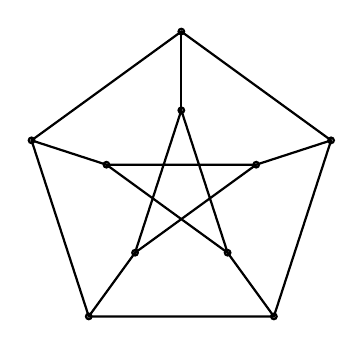
\begin{tikzpicture}[style=thick]
\draw (18:2cm) -- (90:2cm) -- (162:2cm) -- (234:2cm) --
(306:2cm) -- cycle;
\draw (18:1cm) -- (162:1cm) -- (306:1cm) -- (90:1cm) --
(234:1cm) -- cycle;
\foreach \x in {18,90,162,234,306}{
\draw (\x:1cm) -- (\x:2cm);
\draw (\x:2cm) circle (1pt);
\draw (\x:1cm) circle (1pt);
}
\end{tikzpicture}
{$G$}=Petersen graph
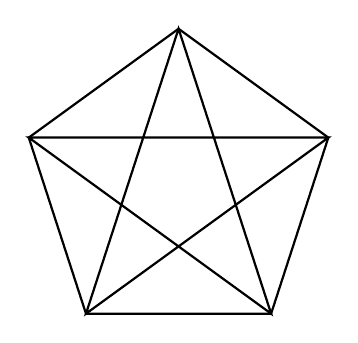
\begin{tikzpicture}[style=thick]
\draw (18:2cm) -- (90:2cm) -- (162:2cm) -- (234:2cm) --
(306:2cm) -- cycle;
\draw (18:2cm) -- (162:2cm) -- (306:2cm) -- (90:2cm) --
(234:2cm) -- cycle;
\foreach \x in {18,90,162,234,306}{}
\end{tikzpicture}
{$K_5$} minor
\end {example}
\begin {remark} If {$G$} is planar then {$G$} has no {$K_5$} or {$K_{3,3}$} subdivision/minor as subgraph
\end {remark}
$(a) \implies (b)$ , $(a) \implies (c)$ are easy implications
\begin {proof} An embedding of {$G$} would contain an embedding of {$K_5$} or {$K_{3,3}$}
\end {proof}
\bigskip
\begin {theorem} (The Four-Color Theorem)
Every planar graph is 4-colorable.
\end {theorem}
\bigskip
\textbf{\textit{Proof history}}
\begin {itemize}
\item 1800-1850 first mentioned
\item 1852 a student of De Morgan conjectured 4-colors are sufficient
\item Cayley popularized it a lot
\item 1879 Alfred Kempe published a proof
\item 1880 Tait had another proof
\item 1890 Heawood found an error in Kempe's proof (but proved the 5-color theorem), 
                  Petersen found an error in Tait's proof
\item 1960 Heesh found a method that could give a proof but involved analysing a huge number of cases
\item 1976 Appel, Haken analysed these cases with a computer ($\approx$ 2000 cases)
\item 1990 Robertson, Seymour and others gave a new computer-assisted proof ($\approx$ 600 cases)
\end {itemize}
\bigskip
\begin {definition} A face is any connected component of ${\rm I\!R^2}$  after removing the embedded graph.
\end {definition}
\begin {observation}\begin{minipage}[t]{\linewidth}
\begin {itemize}
\item There is exactly one unbounded face.
\item Each face is an open subset of ${\rm I\!R^2}$.
\end {itemize}
\end {minipage}
\end {observation}
\begin {observation}
A graph is planar if and only if it can be embedded in ${S^2}$ (the sphere).
Suppose {$G$} is embedded in ${S^2}$.Pick a point of ${S^2}$ not in the embedding.
Use the stereographic projection to map {$G$} onto ${\rm I\!R^2}$.
Note that in a spherical embedding each face is bounded and homeomorphic to an open disk.
\end {observation}
\bigskip
\bigskip
\begin {example} {$Q_3$} as planar graph.
\begin{tikzpicture}[style=thick]
\draw (0,0) -- (2,0) -- (2,2) -- (0,2) -- (0,0)
(0.5,0.5) -- (1.5,0.5) -- (1.5,1.5) -- (0.5,1.5) -- (0.5,0.5)
(0.5,0.5) -- (0,0)
(1.5,0.5) -- (2,0)
(1.5,1.5) -- (2,2)
(0.5,1.5) -- (0,2);
\end {tikzpicture}
\end {example}
\bigskip
\underline{\textbf{Notation}} Suppose I have {$G$} with a fixed planar embedding (or spherical embedding)
\newline
				     {$v$}= \# vertices, {$e$}= \# edges, {$f$}= \# faces.
\begin {theorem}
(Euler's formula) If G is planar and connected, then for any planar embedding of {$G$} :   
$$v-e+f=2.$$
\end {theorem}
\begin {proof}
By induction
\newline
If {$f$}={$1$} then {$G$} has no cycles, as otherwise any cycle of the graph would seperate ${\rm I\!R^2}$ into at $\geq 2$ parts. Hence {$G$} is a tree, $e=v-1$ and
$$v-e+f=v-(v-1)+1=2.$$
If $f\geqslant 2$ then pick an edge $xy\in E(G)$ so that on the two sides of {$xy$} we have two different faces of the embedding.
Now {$G-xy$} is planar, connected and it has 
{$f(G-xy)$}={$f(G)-1$},
{$e(G-xy)$}={$e(G)-1$},
{$v(G-xy)$}={$v(G)$}. 
The proof follows by induction.
\end {proof}
\bigskip
Euler cared about regular polyhedra in ${\rm I\!R^3}$
\newline
\underline{\textbf{Very quick application}}: Classification of Platonic solids (regular polytopes).
\begin {definition} A polytope is regular if:
\begin {enumerate}
\item All vertices have the same degree $k\geqslant3$,
\item All faces are polygons with the same number of sides $l\geqslant3$.
\end {enumerate}
\end {definition}
Let it have {$v$} vertices, {$e$} edges, {$f$} faces in the spherical embedding.

We have these equations:
$\begin{cases}
v-e+f=2\\
kv=2e \\
lf=2e 
\end {cases}$

and so:

$e(\frac{2}{k}-1+\frac{2}{l})=2 \implies \frac{2}{k}+\frac{2}{l}=1+\frac{2}{e}\implies \frac{1}{k}+\frac{1}{l}=\frac{1}{2}+\frac{2}{e}\textgreater \frac{1}{2}$. 

This can be satisfied only for $(k,l)=(3,3),(3,4),(3,5),(4,3),(5,3)$. For each case we uniquely determine $v,e,f$.

\begin{corollary}\begin{minipage}[t]{\linewidth}
Suppose $G$ has at least three vertices.
\begin {enumerate}[(a)]
\item If {$G$} is planar then $e\leqslant3v-6$
\item  If {$G$} is planar and triangle free then $e\leqslant2v-4$
\end {enumerate}
\end {minipage}
\end {corollary}
\begin {proof} We can assume {$G$} is connected. Then $v-e+f=2$.
Count the edges around each face. Each face has length $\geqslant3$ so we get at least ${3f}$.
But each edge is counted twice, so we get exactly $2e$. That means 
$2e\geqslant3f$ or $f\leqslant\frac{2}{3}e$.
\newline
$2=v-e+f\leqslant v-e+ \frac{2}{3}e=v- \frac{1}{3}e$
\newline
$e\leqslant 3v-6$
\newline
If {$G$} is triangle-free then we have a stronger inequality
$2e\geqslant 4f$
and continue the same way.
\end {proof}
\begin {observation} This gives another proof of non-planarity of {$K_{3,3}$} and {$K_5$}
\newline
{$K_5$}: $v=5,e=10$    \: \:\:\:\:\: $10\nleq3\cdot5-6$
\newline
{$K_{3,3}$}: is triangle-free, $v=6, e=9 \: \: \: \: 9\nleq2\cdot6-4$
\end {observation}
\end{document}




